\documentclass{mcmthesis}
\usepackage{indentfirst}
\setlength{\parindent}{2em}
\mcmsetup{CTeX = true,
	tcn = 1919828
	, problem = C,
	sheet = true, titleinsheet = true, keywordsinsheet = true,
	titlepage = true, abstract = true}
\usepackage{palatino}
\usepackage{lipsum}
\title{The \LaTeX{} Template for MCM Version \MCMversion}
\author{}
\date{\today}
\begin{document}
\begin{abstract}
	fhakfhw
	\begin{keywords}
		keyword1; keyword2
	\end{keywords}
\end{abstract}
\maketitle
\tableofcontents

\newpage
\section{Introduction}

\subsection{Background}
In 2016, about 275 million people worldwide used drugs at least once, or 5.6 percent of the world's population aged 15 to 64. About 31 million drug users are suffering from drug addiction, which means their use is so harmful that they may need treatment. Preliminary estimates suggest that 13.8 million young people aged 15 to 16 worldwide used marijuana last year, or 5.6\% of the population.

The world health organization reports that about 450,000 people died from drug use in 2015. Of these deaths, 167,750 were directly related to symptoms of drug use (mainly overdoses). The remaining deaths were indirectly related to drug use, including those from HIV and hepatitis c infection as a result of unsafe injection practices.

The harm caused by opioids continues to be the greatest, accounting for 76 per cent of deaths from drug-related conditions. Injecting drug users --- some 10.6 million people worldwide in 2016 --- bear the greatest health risks; More than half had hepatitis c and one in eight had HIV. Major figures on drug users have changed little in recent years, but this stability masks significant changes taking place in the drug market. Long-term availability of drugs such as heroin and cocaine is increasingly coexisting with new psychoactive substances, as is the non-medical use of prescription drugs (diverted from legal sources or manufactured illegally). Also increasing are the use of substances of unknown origin, which are supplied through illegal channels and are sold claiming to be medicines but destined for non-medical use. The range of substances and compounds available to drug users is unprecedented.\cite{1}

\subsection{Our Work}


\section{Assumptions and Notations}

\subsection{Assumptions}
We make the following basic assumptions in order to simplify the problem. Each
of our assumptions is justified and is consistent with the basic fact.
\begin{itemize}
	\item \textbf{The reported counts contains all the cases of drug use in the states and counties.} There is no unreported drug use case and the report will not lead to a reduction in drug use.
	\item \textbf{The total population of the states and counties remains essentially stable in these years.} The effect of population density on drug use cases is constant.
	\item \textbf{The rest of America and the rest of the world have a constant impact on the five states.} We assume that the external influence on these five states remains the same.
	\item \textbf{States and counties have stable policies on drug use.} We assume that policy does not change during the study period.
\end{itemize}

\subsection{Notations}
The notation table [\ref{table-notations}] contains all the notations we use in this paper.

\begin{table}[h]
	\centering
	\caption{The data example} \label{table-notations}
	\begin{tabular}{cp{20em}}
		\toprule
		ID & 28221526017700008\\
		\hline
		Time & 2018-02-28 22:15:26\\
		\hline
		PayMethod & Cash\\
		\hline
		Price & [0.982] Unit [Hainan Cherry Tomatoes] as [Season Fruit], Origin price [12.90] Discount Price [12.90]\\
		\hline
		isVip & False\\
		\hline
		SolderId & Merchant 22\\
		\bottomrule
	\end{tabular}
\end{table}
\section{}}

\subsection{Graph Theory}
In \textbf(Part 1), we need to describe the spread of the reported cases and identify possible locations where specific opioid use started. From aticle\cite{2}, we learn that weighted directed graph can solve this problem well. The following is the weighted directed graph we constructed. In this diagram [\ref{graph}], each node represents a county and the directed edge W$_{C,D}$ between two nodes C and D represents the influence coefficient of county C on county D is W$_{C,D}$ (The larger the influence coefficient, the more likely the county to be in county c, and the more likely the drug use in county D is to be transmitted from county C). Thus, a graph is constructed for all counties in the five states.
\begin{figure}
	\centering
	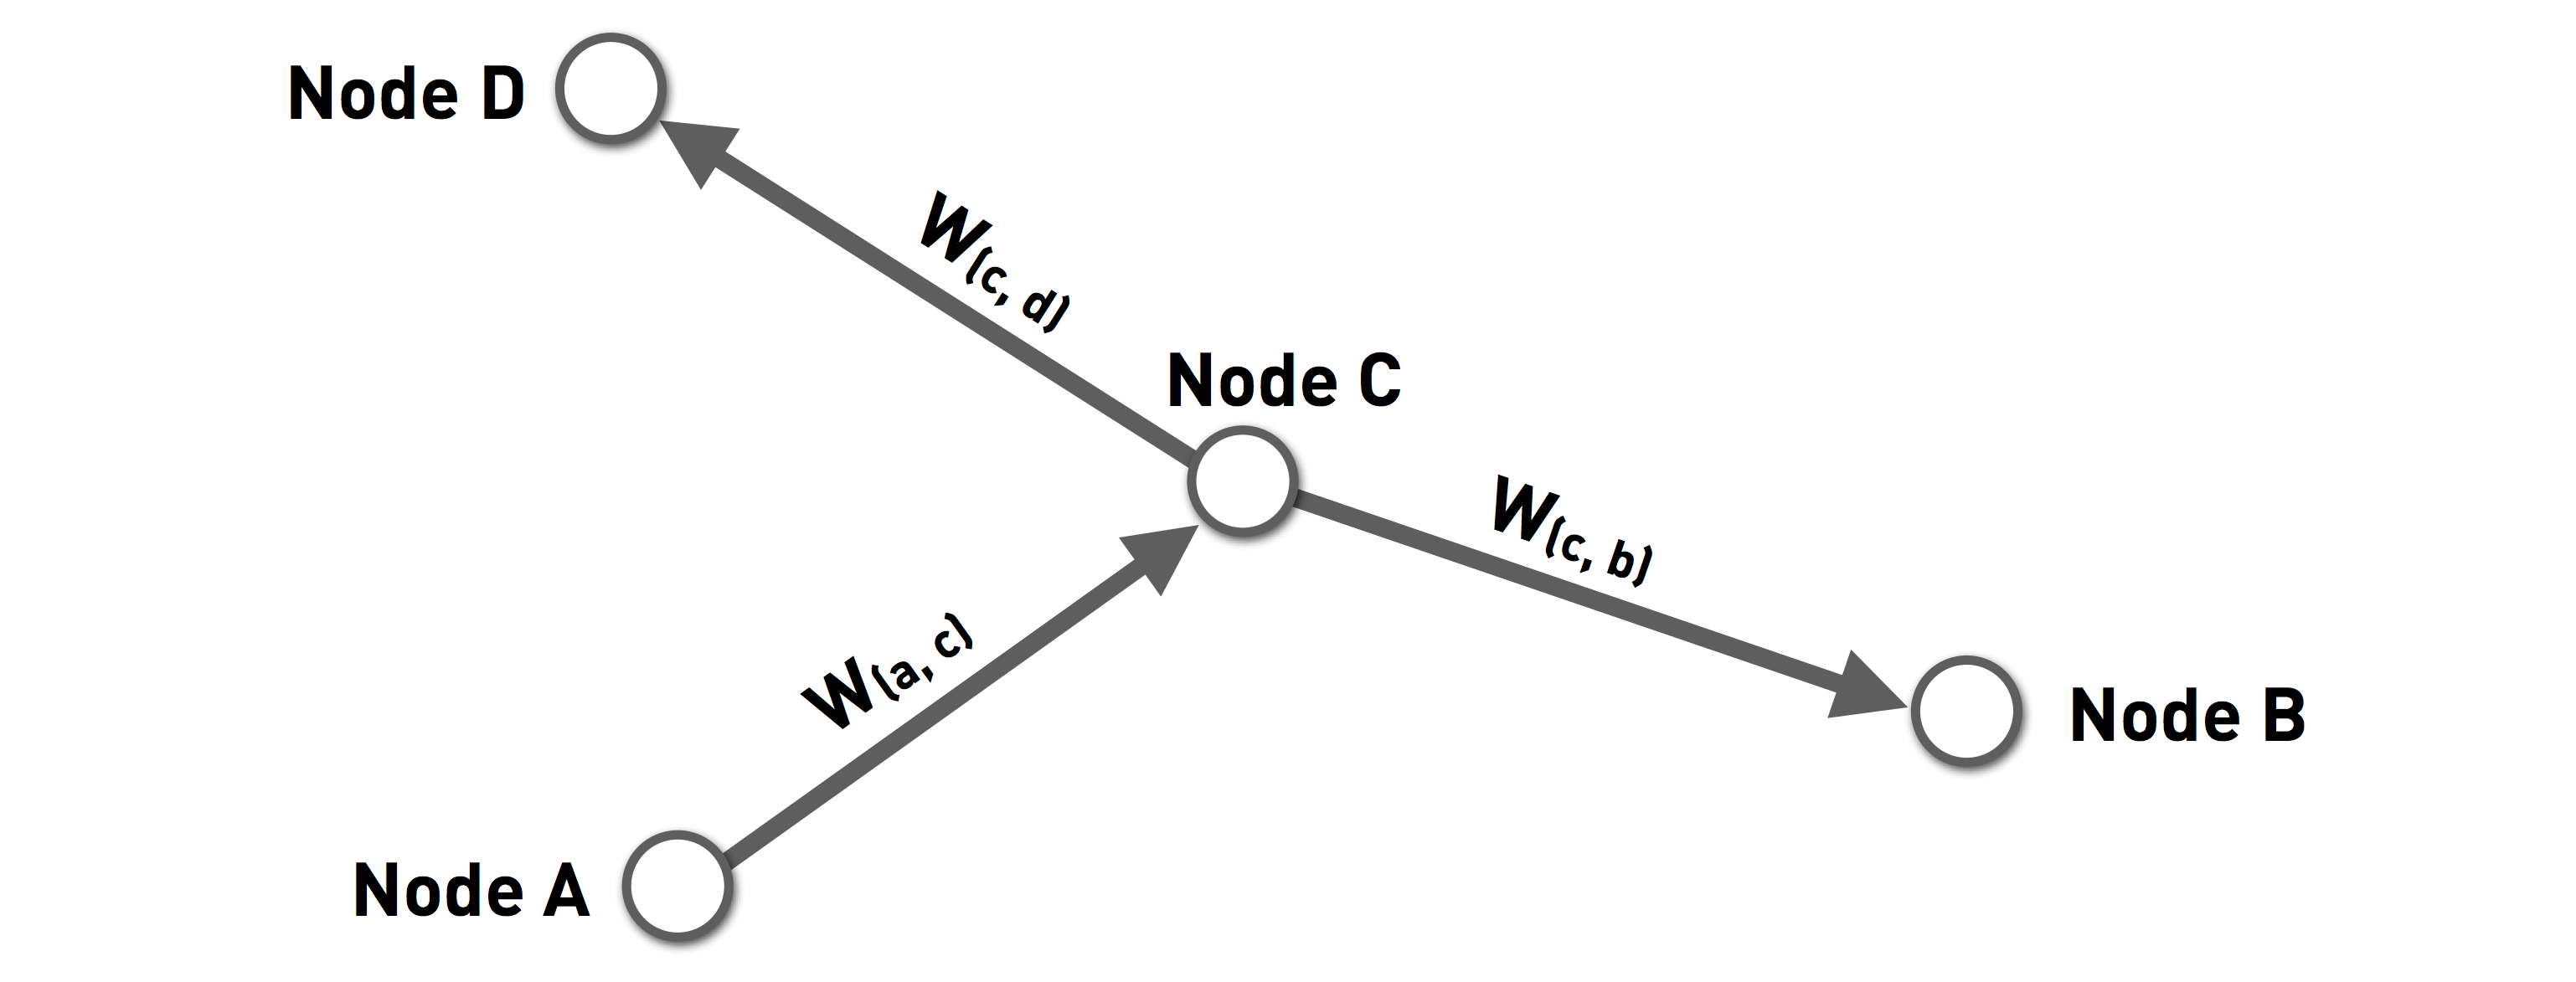
\includegraphics[width=15cm]{graphtheory.png}
	\caption{An Example of the Weighted Directed Graph}\label{graph}
\end{figure}

The advantage of using graph theory analysis is that it can be used to understand the past as well as predict the future. And there are two types of time series: the multiplicative time series and the additive time series.
\begin{itemize}
	\item In a multiplicative time series, the components multiply together to make the time series. If you have an increasing trend, the amplitude of seasonal activity increases. Everything becomes more exaggerated. This is common when you’re looking at web traffic.
	\item In an additive time series, the components add together to make the time series. If you have an increasing trend, you still see roughly the same size peaks and troughs throughout the time series. This is often seen in indexed time series where the absolute value is growing but changes stay relative.
\end{itemize}



So we choose to build the Additive Time Serious Model (ATSM). Here is the reason
\subsection{ARIMA model}
\indent In statistics and econometrics, and in particular in time series analysis, an autoregressive integrated moving average (ARIMA) model is a generalization of an autoregressive moving average (ARMA) model. Both of these models are fitted to time series data either to better understand the data or to predict future points in the series (forecasting). ARIMA models are applied in some cases where data show evidence of non-stationarity, where an initial differencing step (corresponding to the "integrated" part of the model) can be applied one or more times to eliminate the non-stationarity.

The AR part of ARIMA indicates that the evolving variable of interest is regressed on its own lagged (i.e., prior) values. The MA part indicates that the regression error is actually a linear combination of error terms whose values occurred contemporaneously and at various times in the past. The I (for "integrated") indicates that the data values have been replaced with the difference between their values and the previous values (and this differencing process may have been performed more than once). The purpose of each of these features is to make the model fit the data as well as possible.

\subsection{Gause-Lotka-Volterra Model}

\section{Data Analysis}

\subsection{Data Origin}
The major data source is the ``MCM\_NFLIS\_Data.xlsx`` file. It contains all incidents involved with narcotic analgesics and heroin occurring from 2010 to 2017. Hopefully it can figure out the drug crisis spreading amount the northeast U.S.

\subsection{Obvious Factors}
Some factors are provided directly and can be grabbed at the first time:
\begin{itemize}
	\item \textbf{Substances of Drugs}\\
	The main substances of all incidents were provided, hence we may separately analyze them to validate the model.
	\item \textbf{Case Count}\\
	Many drugs involved in all these incidents, but they are not equally significant. The reported count recording the troubles they made can be a convincing factor to determine how influential one drug is.
	\item \textbf{Geography Location}\\
	The specific county name in OH, KY, WV, VA, and PA are provided in detail. Thanks to [Simple Maps Corp.][1] and their generous contribution, we could get accurate longitude and latitude to locate a single county. That would be a great help in visualizing our analysis.
\end{itemize}



\subsection{Error Data Fix}

Some of the purchasing method were mistagged or missed entirely. Those data are either moved in the correct type or in a special "unmarked" type.

Some fruit type are not marked correctly as so, and the similar solution is made, too.

Because of the binary stored float numbers can't be exact, all current numbers (the origin price, discount price, special bonus) are all truncated to 2 digits after the decimal dots.
\section{Model Extension and Simulation Analysis}
\subsection{Problem 1}

\subsubsection{Sensitivity Analysis}

\section{Strengths and weaknesses}

\subsection{Strengths}
\begin{itemize}
	\item \textbf{Applies widely}\\
	This  system can be used for many types of airplanes, and it also
	solves the interference during  the procedure of the boarding
	airplane,as described above we can get to the  optimization
	boarding time.We also know that all the service is automate.
	\item \textbf{Improve the quality of the airport service}\\
	Balancing the cost of the cost and the benefit, it will bring in
	more convenient  for airport and passengers.It also saves many
	human resources for the airline.
\end{itemize}

\subsection{Weaknesses}
\begin{itemize}
	\item
\end{itemize}

\section{Conclusions}
%$ c$_{avg}$ e^{\sin (p+t w)} \left(\frac{\text{C$_{1}$} \text{P$_{1}$}(t)}{\log (\text{D$_{1}$}+1)}+\frac{\text{C$_{2}$} \text{P$_{2}$}(t)}{\log (\text{D$_{2}$}+1)}+\frac{\text{C$_{3}$} \text{P$_{3}$}(t)}{\log (\text{D$_{3}$}+1)}\right)$


\begin{thebibliography}{99}
	\bibitem{1} ``WORLD DRUG REPORT 2018", \url{https://www.unodc.org/wdr2018/prelaunch/}
	\bibitem{2} Boccaletti S, Latora V, Moreno Y, Chavez M, Hwang D U. ``Complex networks: Structure and dynamics". Physics reports, 2006, 424(4): 175-308.
	\bibitem{3}\url{http://www.latexstudio.net/}
	\bibitem{4}\url{http://www.chinatex.org/}
\end{thebibliography}


\begin{appendices}
	
	\section{First appendix}
	
	\lipsum[13]
	
	Here are simulation programmes we used in our model as follow.\\
	
	%\textbf{\textcolor[rgb]{0.98,0.00,0.00}{Input matlab source:}}
	%\lstinputlisting[language=Matlab]{./code/mcmthesis-matlab1.m}
	
	\section{Second appendix}
	
	%some more text \textcolor[rgb]{0.98,0.00,0.00}{\textbf{Input C++ source:}}
	%\lstinputlisting[language=C++]{./code/mcmthesis-sudoku.cpp}
	
	
\end{appendices}
	
	
\end{document}
